\documentclass[letterpaper]{article}

\usepackage{times}
%\usepackage{fullpage}
\usepackage{latexsym}
\usepackage{amsmath}
%\usepackage{hyperref}
\usepackage{graphicx}
\usepackage{aclcite}
\usepackage{alltt}
\usepackage{subfig}

\title{Identifying Lexical Relationships and Subsitutes with Distributional Semantics}
\author{Stephen Roller\\
The University of Texas at Austin\\
{\tt roller@cs.utexas.edu}\\
\\
Doctoral Dissertation Proposal}

\date{\today}

\begin{document}
\maketitle

\begin{abstract}
  As the field of Natural Language Processing has developed, more ambitious
  semantic tasks are starting to be addressed, such as Question Answering, and
  Recognizing Textual Entailment. Systems which approach these tasks can
  perform sophisticated inference between sentences of Natural Language, but
  often have exhibit issues of Montague-style semantics, where the meaning of
  {\em life} is {\em life$'$}. Such systems depend heavily on lexical resources
  like WordNet to provide critical information like the relationships between
  lexical items, or whether one lexical item entails another. However, lexical
  resources are expensive to create and maintain, and can never be
  comprehensive.

  Distributional Semantics has long provided a method to automatically induce
  meaning representations for lexical items from large corpora with little or
  no annotation efforts. In Distributional Semantics, words are modeled as
  vectors in high-dimensional spaces, induced by counting or modeling the
  contexts in which a word appears. The resulting representations are excellent
  as proxies of semantic similarity: words will have similar representations if
  their semantic meanings are similar. Yet, knowing two words are similar does
  not tell us their relationship, or whether one entails the other.

  In this work, we present several techniques for automatically identifying
  specific relationships or entailments from distributional representations of
  lexical semantics. Broadly, this work falls into two distinct but related
  areas: the first predicts specific taxonomic relations and entailment
  decisions between lexical items devoid of context;
  the second predicts specific lexical paraphrases in complete sentences. In
  both cases, we evaluate and emphasize generalization to novel lexical items
  which are devoid of any explicit semantic annotations.  We also provide
  analysis and insight as to how and why these models are anble to generalize
  to novel lexical items, and relate this to prior linguistic and NLP research.

  We propose several short- and long-term extensions to this work. In the
  out-of-context models, we propose applying our model to a broader group of
  lexical relations, and including additional useful features in
  classification.  In the in-context work, we propose extensions which improve
  handling of very rare context items, analyzing the relationships between
  paraphrases. In the long-term, we propose stronger models of in-context
  representations, and unifying the out-of-context and in-context models in
  one of several possible ways.
\end{abstract}

%\pagebreak
\tableofcontents
\pagebreak

%\section*{Table of Contents}
%\begin{itemize}
%  \item Introduction
%    \begin{itemize}
%      \item Distributional Semantics
%      \item Lexical Entailment
%      \item Lexical Substitution
%    \end{itemize}
%  \item Identifying Lexical Relations
%    \begin{itemize}
%      \item Asym (COLING 2014)
%      \item TACL 2016
%    \end{itemize}
%  \item Lexical Substitution
%    \begin{itemize}
%      \item NAACL 2016
%    \end{itemize}
%  \item Proposed Work
%    \begin{itemize}
%      \item 
%    \end{itemize}
%\end{itemize}
%\pagebreak

\section{Introduction}

As the field of Natural Language Processing (NLP) has developed, significant
progress has been made in many areas of research, especially those in ``lower''
levels of the Vauquois Triangle, like Part-of-Speech tagging and Parsing.  Even
difficult semantics tasks, like Sentiment Analysis and Document Classification,
have made significant progress NEEDCITE. Today, there is great deal of emphasis
on sophisticated semantics tasks that require inference and synthesis of
knowledge. These include tasks like Question Answering (QA), where computers
must read and answer questions about passages NEEDCITE, and Recognizing Textual
Entailment (RTE), where computers must decide whether a hypothesis utterance
logically follows from a given text \cite{marelli:2014:semeval}.

Much progress has been made in systems which perform these sort of sophisticated
logical inferences, especially as common benchmarks and data sets have started
to become common \cite{marelli:2014:semeval,bowman:2015:emnlp,needcite}. Yet these
systems ultimately must work over individual lexical items to form a
conclusion, and require knowledge about the relationships between lexical
items. Consider the following example:
\footnote{Mention ``Montague's curse'', as I like to call it?}
\begin{quote}
  Text: The bright girl reads a book.\\
  Hypothesis: The smart child looks at pages of text.
\end{quote}
Any language processing system wishing to infer the second sentence from
the first must know quite a bit of world knowledge: it must know that
girl is a kind of child, and that bright and smart are synonyms in this
context; that books contain pages of text, and that reading involves looking
at some text.

Although significant progress has been made on the text of
Rich Textual Entailment, these systems ultimately depend on some lexical
resources NEEDCITE. The most famous lexical resource is WordNet, which
organizes the lexicon into a large ontology containing many thousands of
annotations of relationships between different lexical items, though countless
other resources also exist and are used (NEEDCITE FrameNet, PPDB, BLESS, LEDS,
SemEval). Unfortunately, resources as thorough as WordNet are extremely
expensive and intensive to create, and since language is ever-changing, they
are inevitably always incomplete, and represent one weak point in Natural
Language Understanding systems. Even modern Neural Network approaches,
which attempt to learn entailments without explicitly depending on these
resources, cannot make entailment predictions about words which were not
in the training data NEEDCITE.

Distributional Semantics offers a potential solution to these issues of lexical
coverage. Distributional Semantics takes inspiration from the famous quote,
``You shall know a word by the company it keeps'' \cite{firth:1957:la}. In
Distributional Semantics, representations of word meaning are automatically
induced by counting or modeling the {\em contexts} in which a word appears.
Distributional Semantics is often sometimes called Vector Space Models (VSM) of
language, as words are represented as vectors a high-dimensional vector space.
Words with similar semantics will have similar vectors in this induced
geometric space. Since VSMs do not require annotated corpora, they are used and
studied as an alternative or predictor of particular lexical resources NEEDCITE.

In this work, we approach the question as to whether Distributional Semantics
can be leveraged to predict some of the lexical inferences necessary in tasks
like RTE. Namely, we present techniques and models for predicting specific
lexical relationships, entailments, and subsitutions using Distributional
Semantics. In Lexical Relationship detection and Entailment detection, we must
predict whether two words exhibit specific relationships, like hypernymy (is-a
relationships) or meronymy (has-a relationships). We present two original
models which can learn to predict hypernymy and sometimes other relations,
and characterize their performance on different data sets, relations. We also
present an original model for Lexical Substitution, in which we must predict a
context-specific synonym for a given target word; we argue that Lexical
Substitution is a form of lexical entailment in context.

Finally, we propose several extensions to this completed work. In the
short-term, we propose drawing a stronger connection between Lexical
Substitution and lexical relationships, analyzing the sort of lexical
relationships which we can and cannot predict in our model. We propose
extending our Lexical Substitution model to better handle out-of-vocabulary
(OoV) issues for very rare context items. We also propose further analysis of
our Lexical Relationship models to see if additional relationships can be
automatically predicted, and consider whether the model can do all-words
relationship prediction.  In the long-term, we wish to consider whether our
Lexical Substitution model can be improved by removing or alleviating a strong
independence assumption in the previous model, and how the Lexical Substitution
and Relationship Detection models could be potentially unified.

\section{Background and Related Work}

\subsection{Distributional Semantics}
%\begin{itemize}
%  \item What is distributional semantics, picture, what is it good for
%  \item How are vectors computed (bow, pmi, dim reduction)
%  \item Dependency vectors, and the importance of col representations
%  \item Important citations: Katrin's survey, Peter's survey
%\end{itemize}

Distributional Semantics is a powerful tool for automatically inducing semantic
representations for lexical items \cite{turney:2010:jair,erk:2012:llc}.  The
core notion is that of the {\em Distributional Hypothesis}, that if two words
appear in similar {\em contexts}, they can be assumed to have similar meaning.
This idea has a long history in the semantics and philosophical literature that
can be traced back over 60 years
\cite{wittgenstein:1953:pi,harris:1954:word,firth:1957:la}. In its modern form,
Distributional Semantics involves finding {\em vector space} representations of
words which are constructed by counting or modeling the contexts in which a
particular word appears. According to the Distributional Hypothesis then, words
with similar vectors can be assumed to have similar meanings
\cite{turney:2010:jair}.

\begin{figure}
\centering
\begin{minipage}{7cm}
\begin{scriptsize}
\begin{alltt}
         the furry {dog} is friendly to
and manipulate the {dog} 's lips and
       as a clever {dog} ; two to
a reputation among {dog} trainers of having
    also among the {dog} breeds most likely
 the very earliest {dog} shows and kennel
        as a guard {dog} and to hunt
   the mechanic 's {dog} began to howl
\end{alltt}
\end{scriptsize}
\end{minipage}\qquad
\begin{minipage}{3cm}
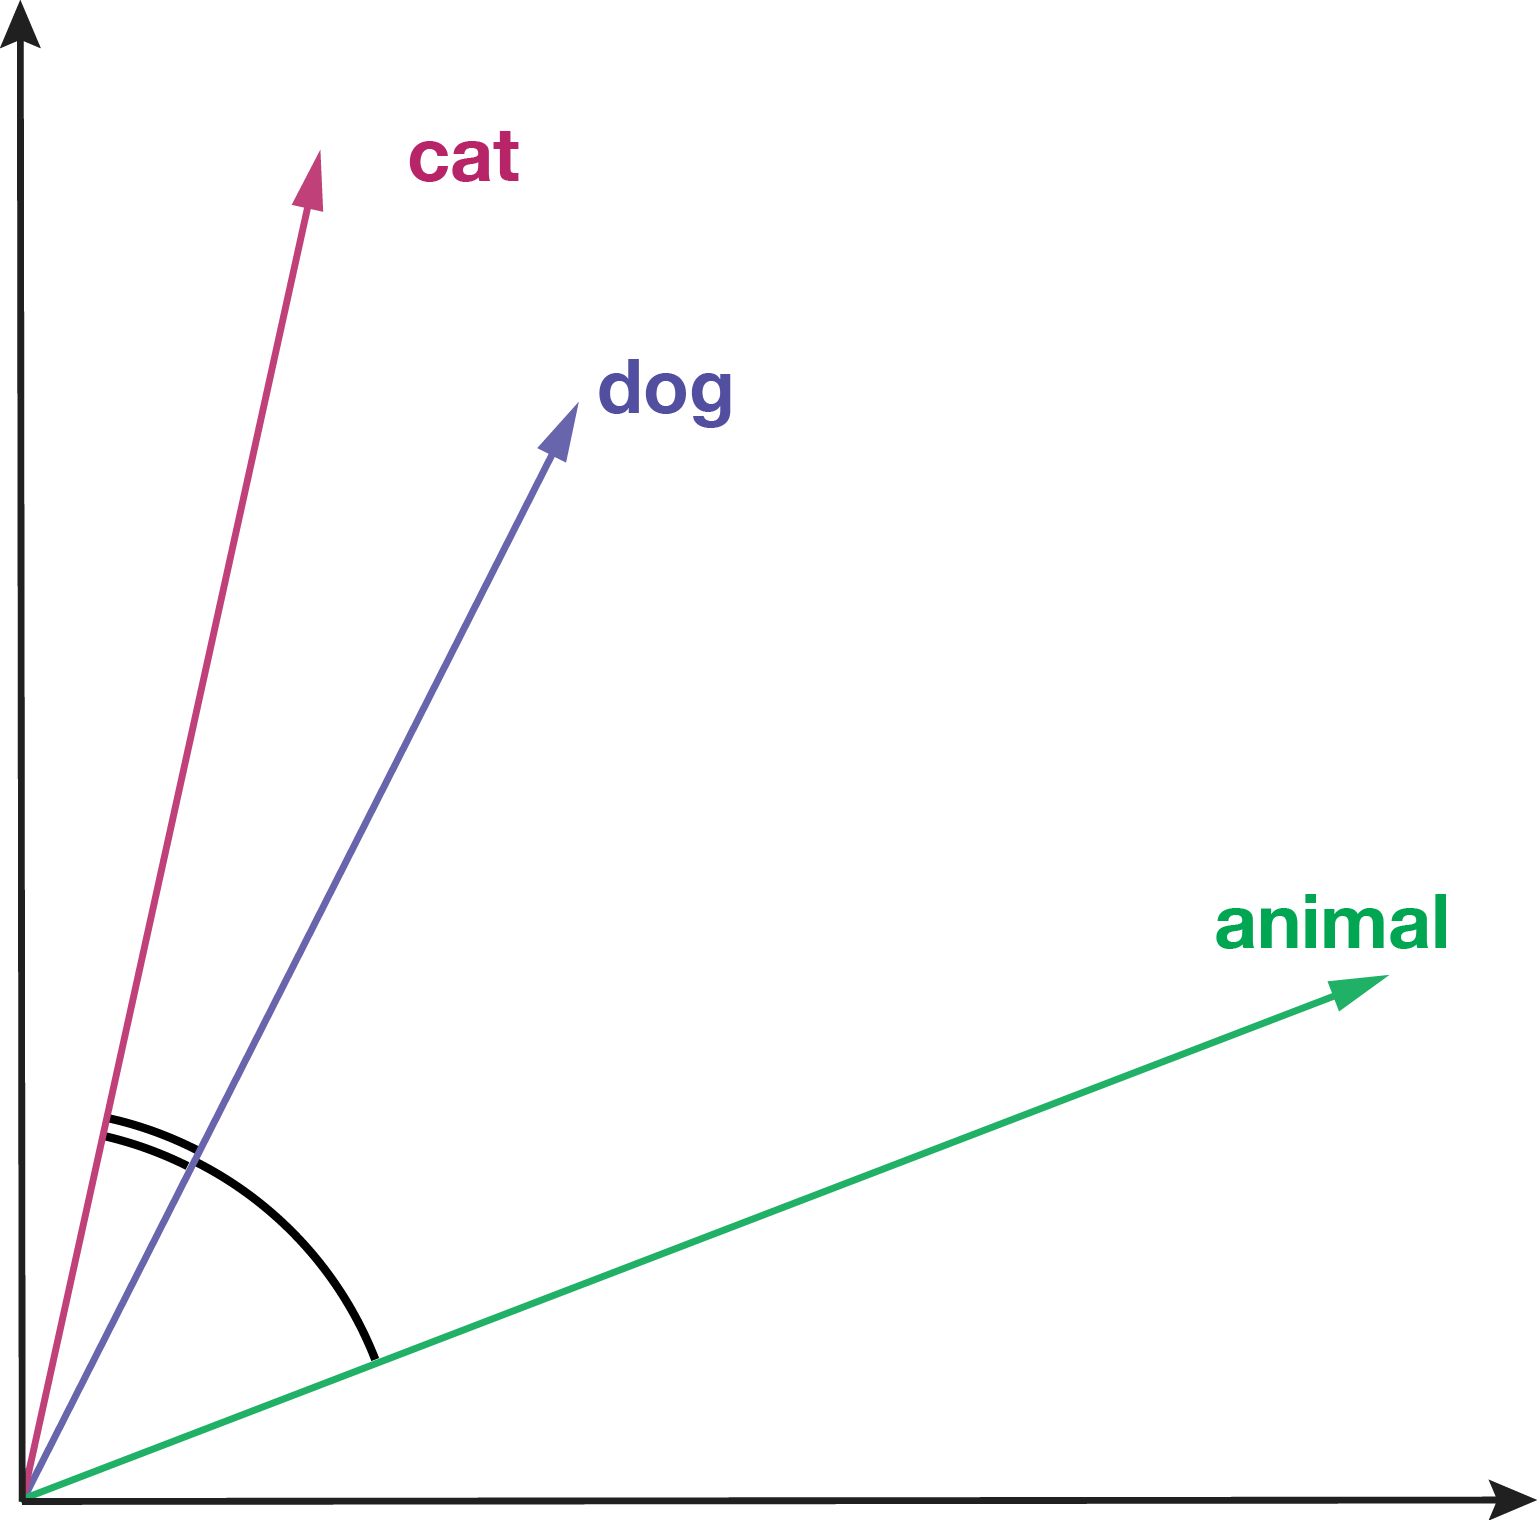
\includegraphics[width=3cm]{figures/vsm}
\end{minipage}
\caption{Contexts of the word {\em dog}, and cartoon drawing
of word vectors.}
\label{fig:vsm}
\end{figure}

In its simplest form, vectors are induced by defining a vector space where
each dimension in the space corresponds to a particular context word. A large,
unannotated corpus of text is then iterated, finding instances of a given word,
like {\em dog}, and incrementing a count for each of the word's {\em
co-occurrences}, or words appearing to the left or right of the target word
{\em dog}, as in Figure~\ref{fig:vsm}. With a large enough corpus, coherent
statistical patterns begin to form. For example, the word {\em furry} is likely
to be used to describe both {\em cat} and {\em dog}, which is then reflected in
the vector counts. After constructing vector representations for the words {\em
cat} and {\em dog}, we can then compare these vectors using {\em cosine
similarity}:
\begin{equation*}
  \text{cosine}(u, v) = \frac{\sum_i u_iv_i}{\sqrt{\sum_i u_i^2 \sum_i v_i^2}}
\end{equation*}
Here, $i$ iterates over all the different context dimensions, like {\em furry}
or {\em kennel}, and cosine similarity is defined over the range of $[0, 1]$.
Words with similar vectors will have a small angle between them, and therefore
a high cosine similarity (e.g. close to 1).

In practice, usually the distributional vectors are more sophisticated in their
construction than raw co-occurrence counts. Typically, words and contexts below
a certain threshold are omitted from the co-occurrence matrix, as extremely
rare words have few counts and therefore impoverished representations. The
co-occurrence matrix is also usually transformed using some non-linearity;
one common choice is Positive Pointwise Mutual Information (PPMI), where the
raw co-occurence count between a word $w$ and context $c$ is transformed,
\begin{equation*}
  \text{PPMI}(w, c) = \max\left(0, \log\frac{P(w, c)}{P(w)P(c)}\right)
\end{equation*}
Pointwise Mutual Information measures roughly how many times more likely
do these two items co-occur more than chance, while Positive PMI additionally
co-occurrences which occur less often than chance. Different transformations,
like Mutual Information, conditional probability, and softplus, are also
sometimes seen in the literature, and each emphasizes different forms of
similarity.

Another important aspect of Distributional Semantics is how context is defined.
In the example of Figure~\ref{fig:vsm}, we showed that context can be defined
as three words to the left and right of the target word, but there are
alternatives. For example, using very large windows of similarity results in
emphasizing more topical similarity, e.g. doctor and hospital, while smaller
windows emphasize more functional similarity, e.g. doctor and surgeon NEEDCITE.
Context can be also defined as {\em syntactic neighbors} extracted
from a dependency parse \cite{pado:2007:cl}. For example, in Figure~\ref{fig:syn},
the contexts for the word {\em chased} would be {\em nsubj+dog} and {\em
dobj+tail}. Distributional Spaces defined in this manner tend to emphasize
the {\em selectional preferences} of words, or the tendency of certain
relations to occur with certain arguments.

\begin{figure}
  \centering
  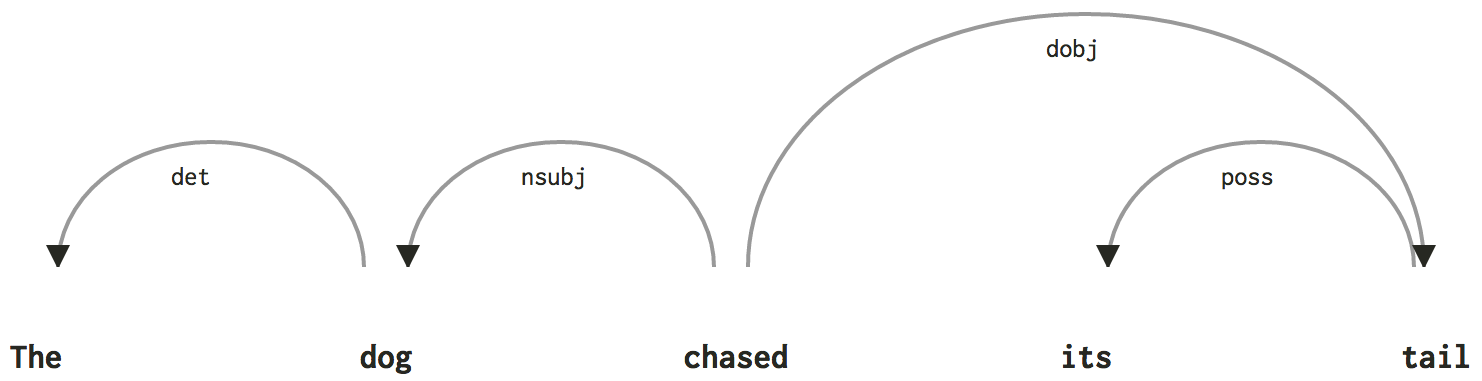
\includegraphics[width=0.75\textwidth]{figures/syn}
\caption{Example of a dependency parse for ``The dog chased its tail.'' In
a syntactic distributional space, the labeled graph edges define contexts
rather than a window.}
\label{fig:syn}
\end{figure}

One final notion in Distributional Semantics we wish to review is that of
dimensionality reduction. As described earlier, the distributional vector
spaces are very high-dimensional; bag-of-words spaces have many thousands of
dimensions (or sometimes as large as the entire vocab, e.g.
\newcite{pennington:2014:emnlp}, while syntactic spaces often have a million
or more dimensions, e.g. \newcite{baroni:2011:gems}. Efficiently dealing
with these large, extremely sparse vectors can sometime be troublesome, so
we often opt to use some form of {\em dimensionality reduction}, like
Singular Value Decomposition \cite{landauer:1997:pr}. In dimensionality
reduction, the co-occurrence matrix $M$ is usually assumed to be factorizable
into two lower-rank matrices,
\begin{equation*}
  M = VC^{\top}
\end{equation*}
where $V$ is some lower dimension representation of word vectors, and $C$
is the corresponding lower dimension representation of the context items.
Interestingly, the recent, popular Word2Vec algorithm \cite{mikolov:2013:iclr}
can also be viewed as a form of dimensionality reduction \cite{levy:2014:nips}.

\subsection{Lexical Entailment}

It can be difficult to give an exact definition of Lexical Entailment, but in
this document we define it as any lexical relationship where a typical,
cooperative reader would logically assume a given consequent from a given
antecedent.\footnote{Katrin, help please!  can you think of something better
with a citation I can use?} This includes many classical lexical relations,
like hypernymy (a girl {\em is a} child; a dog {\em is an} animal), and
meronomy (a girl {\em has} eyes; a dog {has a} tail), but also many
nonclassical ones too. For example, a {\em dissertation} implies a {\em
committee}, but the exact relationship between these items would be difficult
to pigeonhole or generalize to other items.

There has been a great deal of research around predicting lexical entailment
automatically from text; we cannot possibly enumerate all the work on this
problem done in all of NLP, but we aim to cover some influential approaches,
and emphasize attempts to do this with distributional semantics.

One important, early work in this task was that of Hearst patterns
\cite{hearst:1992:coling}, which are specific textual patterns highly
indicative of particular relationships. Common Hearst patterns include
phrases like ``X such as Y,'' ``X including Y,'' which are both highly
indicative of hypernymy; and possessives, like ``X's Y'', can be indicative
of meronomy. In fact, the previous sentence contains several Hearst patterns
{\em about} Hearst patterns. Later, the Hearst pattern method by
\newcite{snow:2004:nips} to include a variety of syntactic patterns rather than
pure textual patterns.

Early work in identify lexical entailments using distributional spaces was
focused mostly on attempts to find unsupervised similarity measures to identify
specific relationships from the word vectors. For hypernymy detection, one
lasting hypothesis has been the Distributional Inclusion Hypothesis
\cite{zhitomirsky-geffet:2005:acl}, which states that the contexts in which a
hypernym appears should be a superset of all its hyponyms, or subordinate
words. Though this seems to be strictly false\footnote{Consider {\em \#The animal
barked loudly at its bowl of animal food.}}, a considerable amount of work has
assumed it to be at least partially true, including our own.


\begin{itemize}
  \item What is Lexical Entailment, how is it defined?
  \item Examples and types of Entailment
    \begin{itemize}
      \item Word relationships (countless kinds)
    \end{itemize}
  \item Linguistic theories, indicators of entailment
  \begin{itemize}
    \item Distributional Inclusion Hypothesis
    \item Hearst Patterns
  \end{itemize}
  \item Works predicting lex entailment using distributional semantics
    \begin{itemize}
      \item Far too extensive to thoroughly cover all groups and models attempting
      to do lexical entailment. Some use vision, some use DS, some explicitly mine
      Wikipedia for phrases, etc
    \end{itemize}
\end{itemize}

\subsection{Lexical Substitution}
\begin{itemize}
  \item What is lexical substitution
  \item Sometimes even more difficult to define that lexical entailment
  \item Linguistic understanding of substitution is less developed
    \begin{itemize}
      \item Violations of selectional preferences?
      \item Synonyms/Entailment in context?
    \end{itemize}
\end{itemize}

\section{Completed work}

\subsection{Hypernymy and Entailment Detection}

\subsubsection{Asym}

\subsubsection{}


\pagebreak
\bibliographystyle{aclcite}
\bibliography{refs}

\end{document}
